\documentclass[12pt]{article}

\usepackage[utf8]{inputenc}
\usepackage{geometry}
\usepackage{graphicx}
\usepackage{array}
\usepackage{fancyhdr}
\usepackage{titlesec}
\usepackage{listings}
\usepackage{xcolor}
\usepackage{amsmath}
\usepackage{hyperref}

\geometry{a4paper, margin=1in}

\setcounter{secnumdepth}{0}

\pagestyle{fancy}
\fancyhf{}

\fancyhead[L]{CSE 2026: Algorithm}
\fancyhead[R]{Algorithm Performance Evaluator}
\renewcommand{\headrulewidth}{0.5pt}

\hypersetup{
    colorlinks=true,
    linkcolor=blue,
    urlcolor=blue,
    citecolor=blue
}

% Code style
\lstset{
    language=Python,
    basicstyle=\ttfamily\small,
    keywordstyle=\color{blue},
    stringstyle=\color{red},
    commentstyle=\color{green!60!black},
    numbers=left,
    numberstyle=\tiny\color{gray},
    breaklines=true,
    frame=single
}

\newcommand{\sectionbreak}{\clearpage}

\begin{document}

% ================= Cover Page =================
\thispagestyle{empty}

\begin{center}

{\large \textbf{Faculty of Engineering --- Zagazig University}}\\
{\large Computer and Systems Engineering Program}\\[0.3cm]
{\small CSE 2026: Algorithm}

\vspace{0.5cm}
\rule{\textwidth}{0.5pt}

\vspace{0.5cm}

{\LARGE \textbf{Algorithm Performance Evaluator}}

\vspace{0.5cm}

\rule{\textwidth}{0.5pt}

\vspace{1cm}

{\large \textit{Project Report}}

\vspace{1cm}

\end{center}

\begin{center}
\renewcommand{\arraystretch}{1.5}
\begin{tabular}{|p{4.5cm}|p{6cm}|p{5cm}|}
\hline
\textbf{Name} & \textbf{E-mail} & \textbf{Work} \\
\hline

Youssef Reda & youssefreda866@gmail.com & Back-End \\
\hline
Mohamed Moustafa & mo8729\_11@outlook.com & API Client \\
\hline
Ali Mohamed & aly200565@gmail.com & Dashboard \\
\hline
Mohamed Ali & m7md3ly2712005@gmail.com & Dashboard Controller \\
\hline

\end{tabular}
\end{center}

\vfill

\begin{center}
Academic Year 2025/2026
\end{center}

\newpage

% ================= TOC =================
\thispagestyle{empty}
\tableofcontents
\newpage

% ================= Sections =================

\section{Overview}

% \thispagestyle{empty}

The Algorithm Performance Evaluator is a desktop application designed to bridge the gap between theoretical Big O analysis and practical execution. It allows users to input custom algorithm implementations and evaluate their behavior under real execution conditions.

The system runs the provided code on dynamically generated inputs of different sizes, measures execution time, and analyzes performance trends to estimate the algorithm's time complexity automatically.

Unlike traditional analysis that depends only on theoretical models such as $O(n)$ and $O(n \log n)$, this application focuses on empirical evaluation, taking into account real execution factors such as implementation details and input variations.

The system consists of a back-end responsible for execution, timing, and analysis, and a front-end that provides a clear interface for displaying results.

\section{Core Functionality}

% \thispagestyle{empty}

\subsection{Code Interface}

The Code Interface provides a dedicated area where users can write their algorithm inside a predefined function template. The function receives an array as input, ensuring a consistent format for all executions.

This structure allows the system to automatically generate test cases and pass them to the user’s code without additional setup. It helps users focus on implementing the algorithm logic while reducing input-related errors.

The interface is directly connected to the execution engine, enabling the written code to be tested and analyzed within the system.

\vspace{1cm}
\subsection{Complexity Estimation Engine}

The Complexity Estimation Engine is responsible for automatically identifying the time complexity class that best matches the algorithm’s performance. It analyzes execution time across varying input sizes and detects the growth pattern of the algorithm.
Based on this analysis,\\
the system classifies the algorithm into standard complexity categories such as

\begin{itemize}
\item $O(1)$ - Constant
\item $O(n)$ - Linear
\item $O(n \log n)$ - Linearithmic
\item $O(n^2)$ - Quadratic
\item $O(n^3)$ - Cubic
\item $O(n^2 \log n)$
\item $O(2^n)$ - Exponential
\item ...and others.
\end{itemize}

\section{System Architecture}

The system architecture of the Algorithm Performance Evaluator is designed to ensure a clear separation between processing logic and user interaction
The application is divided into two main components: 
a back-end responsible for computation and analysis, 
and a front-end responsible for user interaction and visualization.\\

The back-end handles tasks such as input generation, code execution, runtime measurement, and complexity analysis.\\
On the other hand, the front-end provides an intuitive interface that allows users to input their code, control execution modes, 
and view results in a clear and interactive manner.\\

This separation improves system organization, scalability, and maintainability, making it easier to extend and manage the application.

\vspace{1cm}
\begin{figure}[h]
\centering
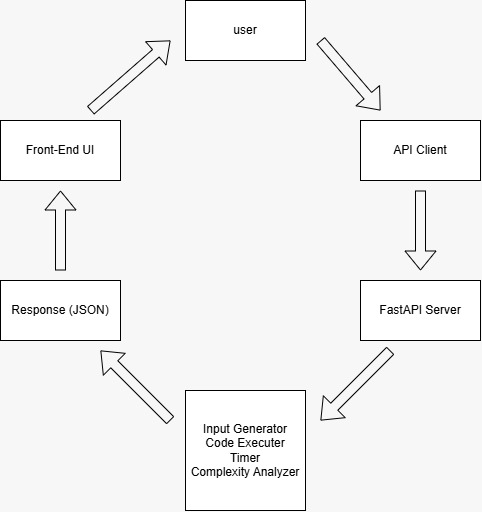
\includegraphics[width=0.8\textwidth]{../Assets/Architecture.jpeg}
\caption{System Architecture Diagram}
\end{figure}

\vspace{1cm}
\subsection{Back-End}

The back-end is responsible for handling the core processing tasks of the system. It manages the workflow of executing the user-defined algorithm, generating input data, measuring runtime, and analyzing performance.

It is designed in a modular way, where each component performs a specific function, ensuring better organization and easier maintenance.

\vspace{1cm}
\subsubsection{Schemas}

The Schemas component defines the data structures used for communication between different parts of the system. It ensures that input data, execution requests, and analysis results follow a consistent and organized format.

These schemas are used to validate incoming data and structure the output returned by the back-end, making the system more reliable and easier to maintain.\\

\newpage
\textbf{Code}

\begin{lstlisting}
from pydantic import BaseModel, Field
from typing import List, Optional, Literal

# REQUEST
class AnalysisRequest(BaseModel):
    code : str
    array: Optional[str] = None
    size : Optional[str] = None
    mode : Literal["MANUAL", "AUTO"]

# CHART POINT
class ChartPoint(BaseModel):
    n   : int
    time: float

# CANDIDATE CLASS
class Candidate(BaseModel):
    name : str     
    score: float  

# RESPONSE
class AnalysisResponse(BaseModel):
    complexity       : str
    description      : str
    confidence       : float
    candidates       : List[Candidate]  = Field(default_factory=list)
    best_chart_data  : List[ChartPoint] = Field(default_factory=list)
    avg_chart_data   : List[ChartPoint] = Field(default_factory=list)
    worst_chart_data : List[ChartPoint] = Field(default_factory=list)
    best             : str
    avg              : str
    worst            : str
\end{lstlisting}

\newpage
\subsubsection{Input Generator}

The Input Generator is responsible for creating test data of varying sizes to evaluate algorithm performance. It generates different types of inputs, including random, sorted, and reversed arrays, to test the algorithm under multiple scenarios.

Additionally, it adapts input sizes based on the algorithm’s initial execution speed, ensuring efficient and meaningful performance evaluation.

\vspace{1cm}
\textbf{Code}

\begin{lstlisting}
import random

class InputGenerator:
 
    def get_adaptive_sizes(self, probe_time: float) -> list[int]:
        if probe_time < 0.1:
            return [5000, 10000, 20000, 30000, 50000]
 
        elif probe_time < 1.0:
            return [1000, 2000, 3000, 5000, 8000, 10000]
 
        elif probe_time < 10.0:
            return [500, 1000, 1500, 2000, 2500, 3000]
 
        else:
            return [100, 200, 300, 500, 700, 1000]
    
    def generate_random(self, n: int) -> list[int]:
        if n <= 0:
            raise ValueError("Size_must_be_positive")
        return [random.randint(1, 1000) for _ in range(n)]

    def generate_sorted(self, n: int) -> list[int]:
        if n <= 0:
            return []
        return list(range(1, n + 1))

    def generate_reversed(self, n: int) -> list[int]:
        if n <= 0:
            return []
        return list(range(n, 0, -1))

    def parse_array(self, array_str: str) -> list[int]:
        if not array_str.strip():
            return []
        try:
            return [int(x) for x in array_str.strip().split()]
        except ValueError:
            raise ValueError("Invalid_array_input.Use_space-separated_integers.")

\end{lstlisting}

\newpage
\subsubsection{Code Executor}

The Code Executor is responsible for safely running the user-defined algorithm within a controlled environment. It executes the provided code, passes the generated input to the algorithm, and returns the result for further analysis.

To ensure reliability and security, the execution is performed using a restricted set of built-in functions, preventing unsafe operations. The system also validates the presence of the required function and handles runtime errors gracefully.

\vspace{1cm}
\textbf{Code}

\begin{lstlisting}
import traceback

class CodeExecutor:

    def execute(self, code: str, arr: list[int]) -> list[int]:
        safe_globals = {"__builtins__": self._safe_builtins()}
        local_vars   = {"arr": arr.copy()}

        try:
            exec(code, safe_globals, local_vars)
        except Exception as e:
            raise RuntimeError(f"Code_execution_error:\n{traceback.format_exc()}")

        if "my_algorithm" not in local_vars:
            raise RuntimeError(
                "Function_'my_algorithm'_not_found!\n"
                "Please_define_your_algorithm_as:\n"
                "def my_algorithm(arr):\n"
                "    ...")

        try:
            result = local_vars["my_algorithm"](arr.copy())
        except Exception as e:
            raise RuntimeError(f"Error running my_algorithm:\n{traceback.format_exc()}")

        return result

    # SAFE BUILTINS -- Here
\end{lstlisting}

\newpage
\subsubsection{Timer}

The Timer component is responsible for measuring the execution time of the algorithm with high precision. It uses a performance-based clock to calculate the runtime in milliseconds for accurate evaluation.

To improve measurement reliability, the system executes the algorithm multiple times and computes a representative value by removing outliers and taking the median. It also performs an initial warm-up run to stabilize execution performance.

This approach ensures consistent and accurate timing results, which are essential for analyzing performance trends and estimating complexity.

\vspace{1cm}
\textbf{Code}

\begin{lstlisting}
import time
import statistics
import traceback
from executor.code_executor import CodeExecutor

class Timer:

    def __init__(self):
        self.executor = CodeExecutor()

    def measure(self, code: str, arr: list[int]) -> float:        
        start = time.perf_counter()
        self.executor.execute(code, arr)
        end   = time.perf_counter()

        time_ms = (end - start) * 1000
        return time_ms

    def measure_average(self, code: str, arr: list[int], runs: int = 5) -> float:
        try :
            # Warm Up 
            self.executor.execute(code, arr)

            times = []
            for _ in range(runs):
                t = self.measure(code, arr)
                times.append(t)

            # Remove min and max then -> take median
            times.sort()
            trimmed = times[1:-1] if len(times) > 3 else times
            return round(statistics.median(trimmed), 4)

        except Exception as e:
            raise RuntimeError(f"Measurement_failed_at_n={len(arr)}:\n{traceback.format_exc()}")
\end{lstlisting}

\newpage
\subsubsection{Complexity Analyzer}

The Complexity Analyzer is responsible for estimating the time complexity of the algorithm based on empirical execution data. It compares the measured runtime against a set of predefined complexity functions and determines which model best fits the observed growth pattern.

The system evaluates multiple candidate functions such as constant, logarithmic, linear, and polynomial complexities. For each function $f(n)$, it computes the ratio between the measured time and the expected growth:

$$
\text{ratio} = \frac{T(n)}{f(n)}
$$

To ensure stability, the analyzer calculates the coefficient of variation (CV) of these ratios:

$$
CV = \frac{\sigma}{\mu}
$$

where $\mu$ is the mean and $\sigma$ is the standard deviation. A lower CV indicates a better fit between the function and the observed data.

The system then assigns a confidence score to each candidate and selects the complexity with the highest score as the final result.


\vspace{1cm}
\textbf{Code}

\begin{lstlisting}
import math

class ComplexityAnalyzer:

    def analyze(self, results: list[dict]) -> dict:
        if len(results) < 2:
            return self._build_result("O(n)", 0.5, [])
        
        cv_map = {}
        for name, func in self.FUNCTIONS.items():
            cv = self._coefficient_of_variation(func, results)
            cv_map[name] = cv

        candidates = self._build_candidates(cv_map)

        if not candidates:
            return self._build_result("O(n)", 0.5, [])

        best_match = candidates[0]["name"]
        confidence = candidates[0]["score"]

        return self._build_result(best_match, confidence, candidates)

    def _coefficient_of_variation(self, func, results: list[dict]) -> float:
        ratios = []
        for r in results:
            n    = r["n"]
            time = r["time"]
            f    = func(n)
            if f > 0 and time > 0:
                ratios.append(time / f)

        if len(ratios) < 3:
            return float("inf")
        
        ratios.sort()
        trim = max(1, len(ratios) // 10)
        trimmed_ratios = ratios[trim:-trim] if len(ratios) > 5 else ratios

        mean = sum(trimmed_ratios) / len(trimmed_ratios)
        if mean == 0:
            return float("inf")

        std_dev = math.sqrt(sum((r - mean) ** 2 for r in trimmed_ratios) / len(trimmed_ratios))

        return std_dev / mean

    def _build_candidates(self, cv_map: dict) -> list[dict]:
        finite_cvs = {name: cv for name, cv in cv_map.items()
                      if cv != float("inf")}

        if not finite_cvs:
            return []
        
        max_cv = max(finite_cvs.values())
        if max_cv == 0:
            return []

        candidates = []
        for name, cv in finite_cvs.items():
            score = round(1.0 - (cv / max_cv), 3)
            score = max(0.0, min(1.0, score))
            candidates.append({
                "name" : name,
                "score": score
            })

        candidates.sort(key=lambda x: x["score"], reverse=True)
        return candidates
\end{lstlisting}

\newpage
\subsubsection{FastAPI Endpoint}

The FastAPI Endpoint serves as the interface between the front-end and the back-end system. It receives user requests, processes the submitted algorithm, and returns the analysis results in a structured format.

The main endpoint accepts the user code and execution mode, then coordinates different components such as the input generator, timer, and complexity analyzer to perform the evaluation. It supports both manual and automatic modes, allowing flexible testing scenarios.

The system also includes validation and error handling mechanisms to ensure reliable communication and proper response formatting.

\vspace{1cm}
\textbf{Part of Code}

\begin{lstlisting}
@app.get("/")
def health_check():
    return {"status": "running", "message": "Algorithm Performance Evaluator API"}

@app.post("/analyze", response_model=AnalysisResponse)
def analyze(request: AnalysisRequest):

    try:
        probe_time = probe_speed(request.code)
        sizes      = generator.get_adaptive_sizes(probe_time)

        if request.mode == "MANUAL":
            arr     = generator.parse_array(request.array)
            time_ms = timer.measure_average(request.code, arr)

            results, best_results, worst_results,best_chart_data, avg_chart_data, worst_chart_data = run_benchmark(request.code, sizes)

            if len(arr) >= 100:
                results.insert(0,       {"n": len(arr), "time": time_ms})
                best_results.insert(0,  {"n": len(arr), "time": time_ms})
                worst_results.insert(0, {"n": len(arr), "time": time_ms})

            avg_chart_data.insert(0,   ChartPoint(n=len(arr), time=time_ms))
            best_chart_data.insert(0,  ChartPoint(n=len(arr), time=time_ms))
            worst_chart_data.insert(0, ChartPoint(n=len(arr), time=time_ms))
\end{lstlisting}

\newpage
\subsection{Front-End}

The front-end is responsible for providing a user-friendly interface that allows users to interact with the system. It is implemented using JavaFX, enabling the creation of a responsive and visually structured desktop application.

The interface allows users to input their algorithms, control execution modes, and visualize the analysis results. It communicates with the back-end through API requests and presents the returned data in a clear and interactive way, improving the overall user experience.

\vspace{0.5cm}
\subsubsection{Dashboard}

The Dashboard represents the main user interface of the application. It provides a structured layout that allows users to input their algorithms, control execution modes, and view analysis results.

The interface is divided into key sections, including an input panel for writing code, a control panel for selecting execution options, and a results panel for displaying performance metrics and complexity analysis.

The design focuses on clarity and usability, ensuring that users can interact with the system and understand the results.

\begin{figure}[h]
    \centering
    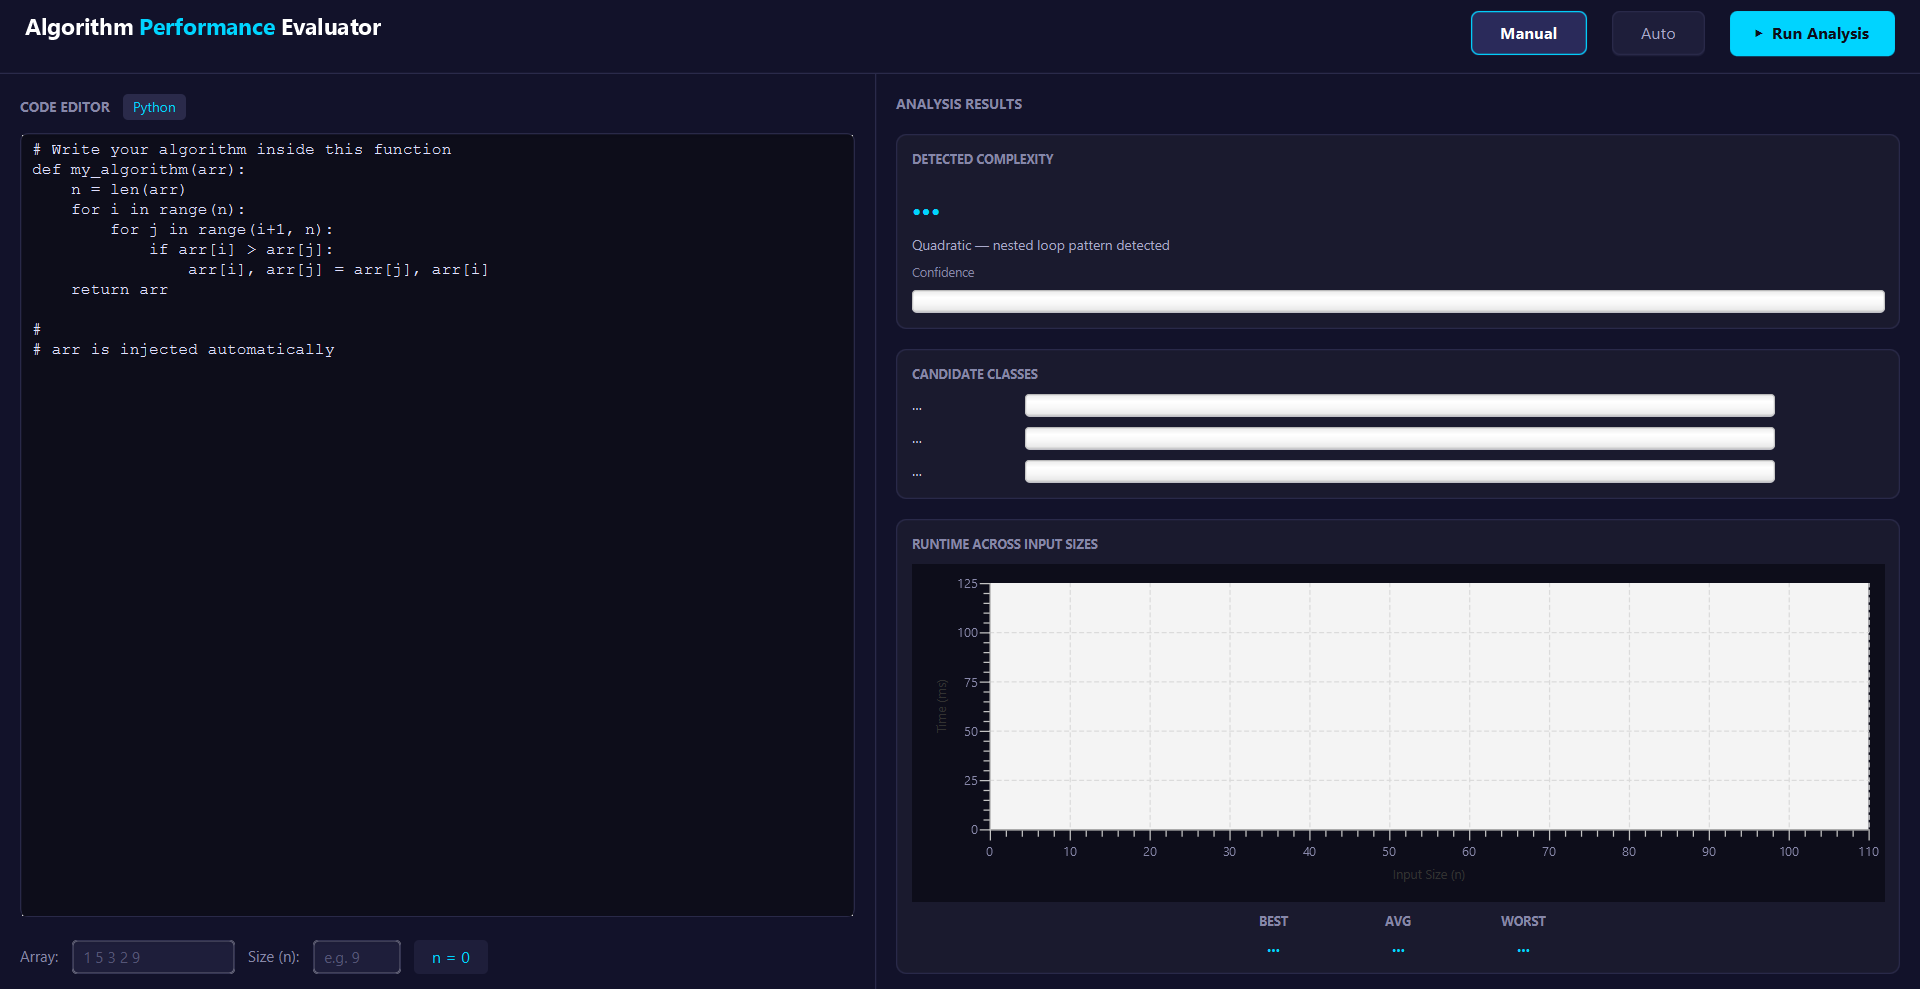
\includegraphics[width=0.9\textwidth]{../Assets/Dashboard.png}
    \caption{Dashboard Interface}
\end{figure}

\newpage
\subsubsection{Dashboard Controller}

The Dashboard Controller manages the interaction between the user interface and the back-end system. It handles user actions such as submitting code, selecting execution modes, and triggering analysis requests.

It is also responsible for receiving the results from the API and updating the interface components accordingly, ensuring a smooth and responsive user experience.

\vspace{1cm}
\subsubsection{Analysis Response}

The Dashboard Controller manages the interaction between the user interface and the back-end system. It handles user actions such as submitting code, selecting execution modes, and triggering analysis requests.

It is also responsible for receiving the results from the API and updating the interface components accordingly, ensuring a smooth and responsive user experience.

\newpage
\subsubsection{API Client}

The API Client is responsible for handling communication between the front-end application and the back-end server. It sends user requests to the API and receives the analysis results in JSON format.

\begin{itemize}
\item \textbf{Request Handling:} The client builds an HTTP POST request containing the user code, input data, and execution mode. The request is formatted as JSON and sent to the back-end endpoint.

\item \textbf{Response Processing:} After receiving the server response, the client checks the status code and converts the returned JSON data into an AnalysisResponse object used within the application.

\item \textbf{Networking and Configuration:} The client uses Java's HttpClient with a defined timeout to ensure reliable communication, along with the Gson library for JSON serialization and deserialization.
\end{itemize}

\vspace{1cm}
\textbf{Part of Code}

\begin{lstlisting}[language=Java]
    public AnalysisResponse analyze(String code, String arrayInput,
                                     String sizeInput, String mode) throws Exception {

        // Build request body
        AnalysisRequest requestBody = new AnalysisRequest(code, arrayInput, sizeInput, mode);
        String jsonBody = gson.toJson(requestBody);

        System.out.println("JSON: " + jsonBody);

        // Build HTTP POST request 
        HttpRequest request = HttpRequest.newBuilder()
                .uri(URI.create(BASE_URL + "/analyze"))
                .header("Content-Type", "application/json")
                .timeout(Duration.ofSeconds(TIMEOUT))
                .POST(HttpRequest.BodyPublishers.ofString(jsonBody))
                .build();

        // Send request and get response 
        HttpResponse<String> response = httpClient.send(
                request,
                HttpResponse.BodyHandlers.ofString(java.nio.charset.StandardCharsets.UTF_8));

        // Convert JSON response -- AnalysisResponse object
        return gson.fromJson(response.body(), AnalysisResponse.class);
    }    
\end{lstlisting}

\section{Test Results}

\subsection{Bubble Sort}

\textbf{Code}
\begin{lstlisting}
    def my_algorithm(arr):
    arr = arr.copy()
    n = len(arr)
    for i in range(n):
        for j in range(0, n - i - 1):
            if arr[j] > arr[j + 1]:
                arr[j], arr[j + 1] = arr[j + 1], arr[j]
    return arr
\end{lstlisting}

\vspace{0.5cm}
\textbf{Result}
\begin{figure}[h]
    \centering
    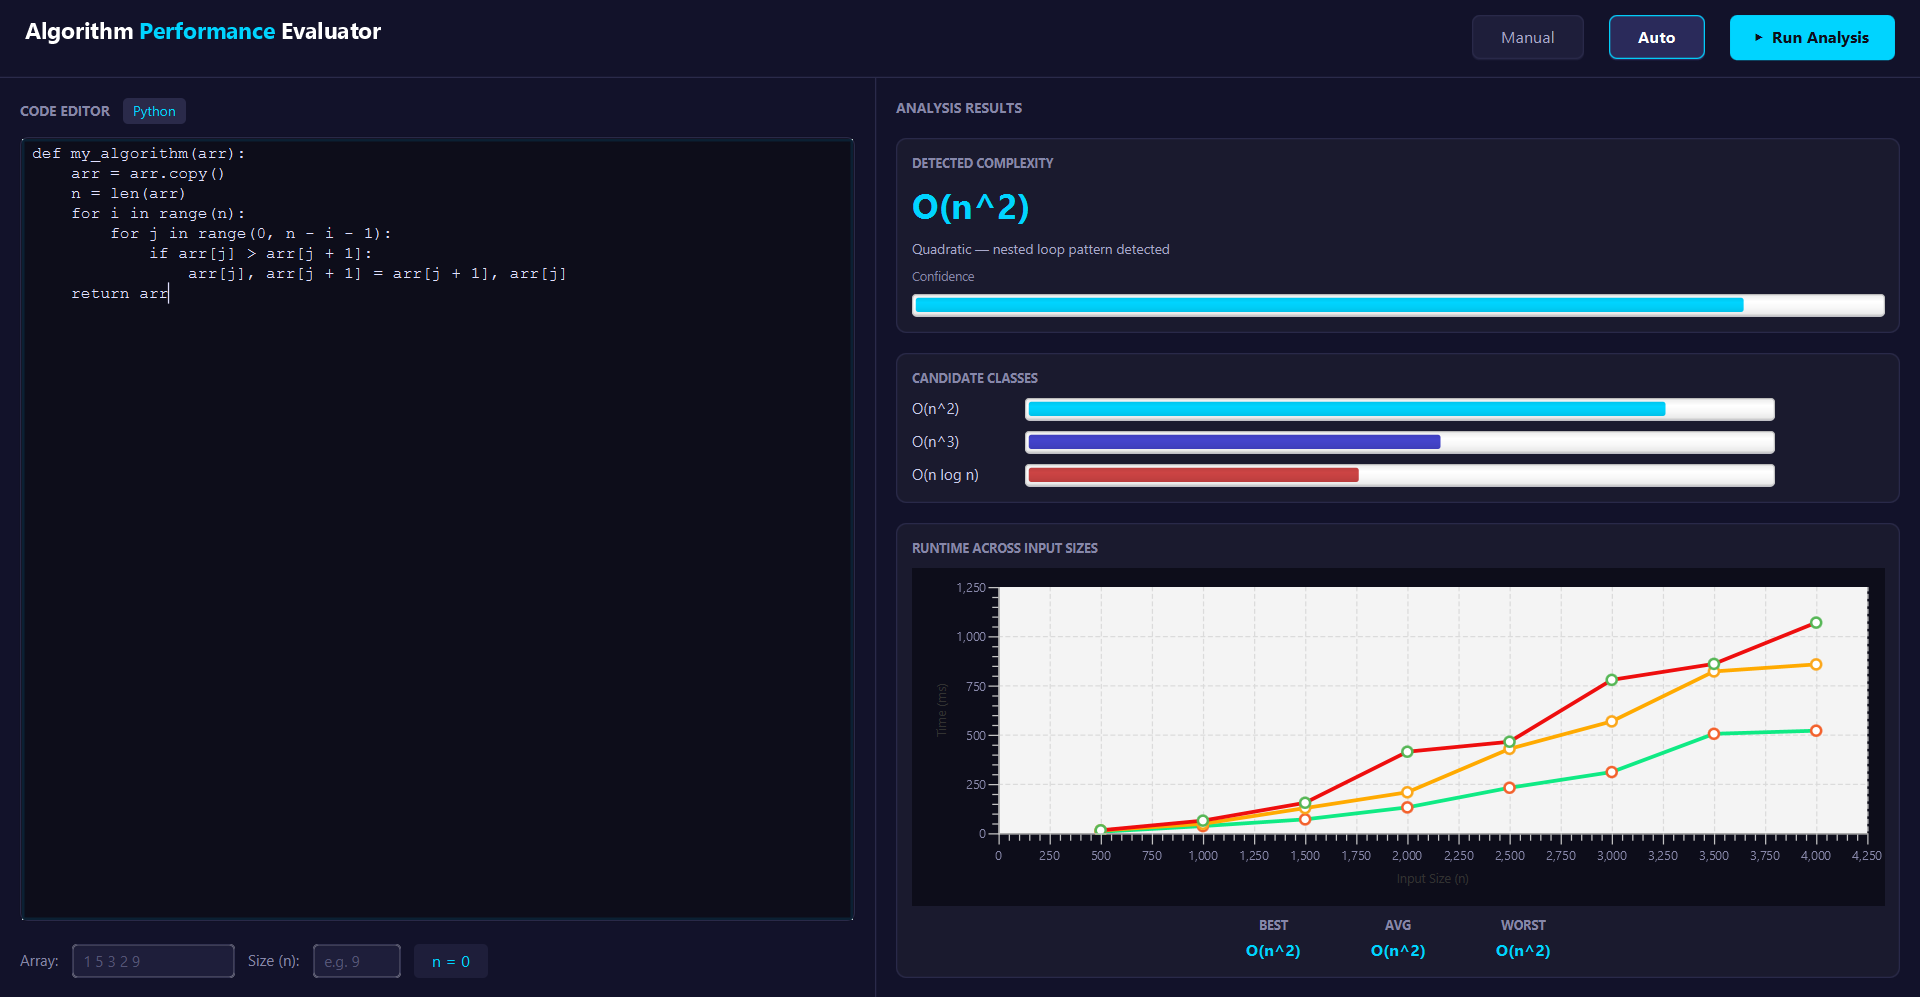
\includegraphics[width=0.9\textwidth]{../Assets/Bubble_Sort.png}
    \caption{Bubble Sort}
\end{figure}

\newpage
\subsection{Insertion Sort}

\textbf{Code}
\begin{lstlisting}
    def my_algorithm(arr):
    arr = arr.copy()
    for i in range(1, len(arr)):
        key = arr[i]
        j = i - 1
        while j >= 0 and arr[j] > key:
            arr[j + 1] = arr[j]
            j -= 1
        arr[j + 1] = key
    return arr
\end{lstlisting}

\vspace{0.5cm}
\textbf{Result}
\begin{figure}[h]
    \centering
    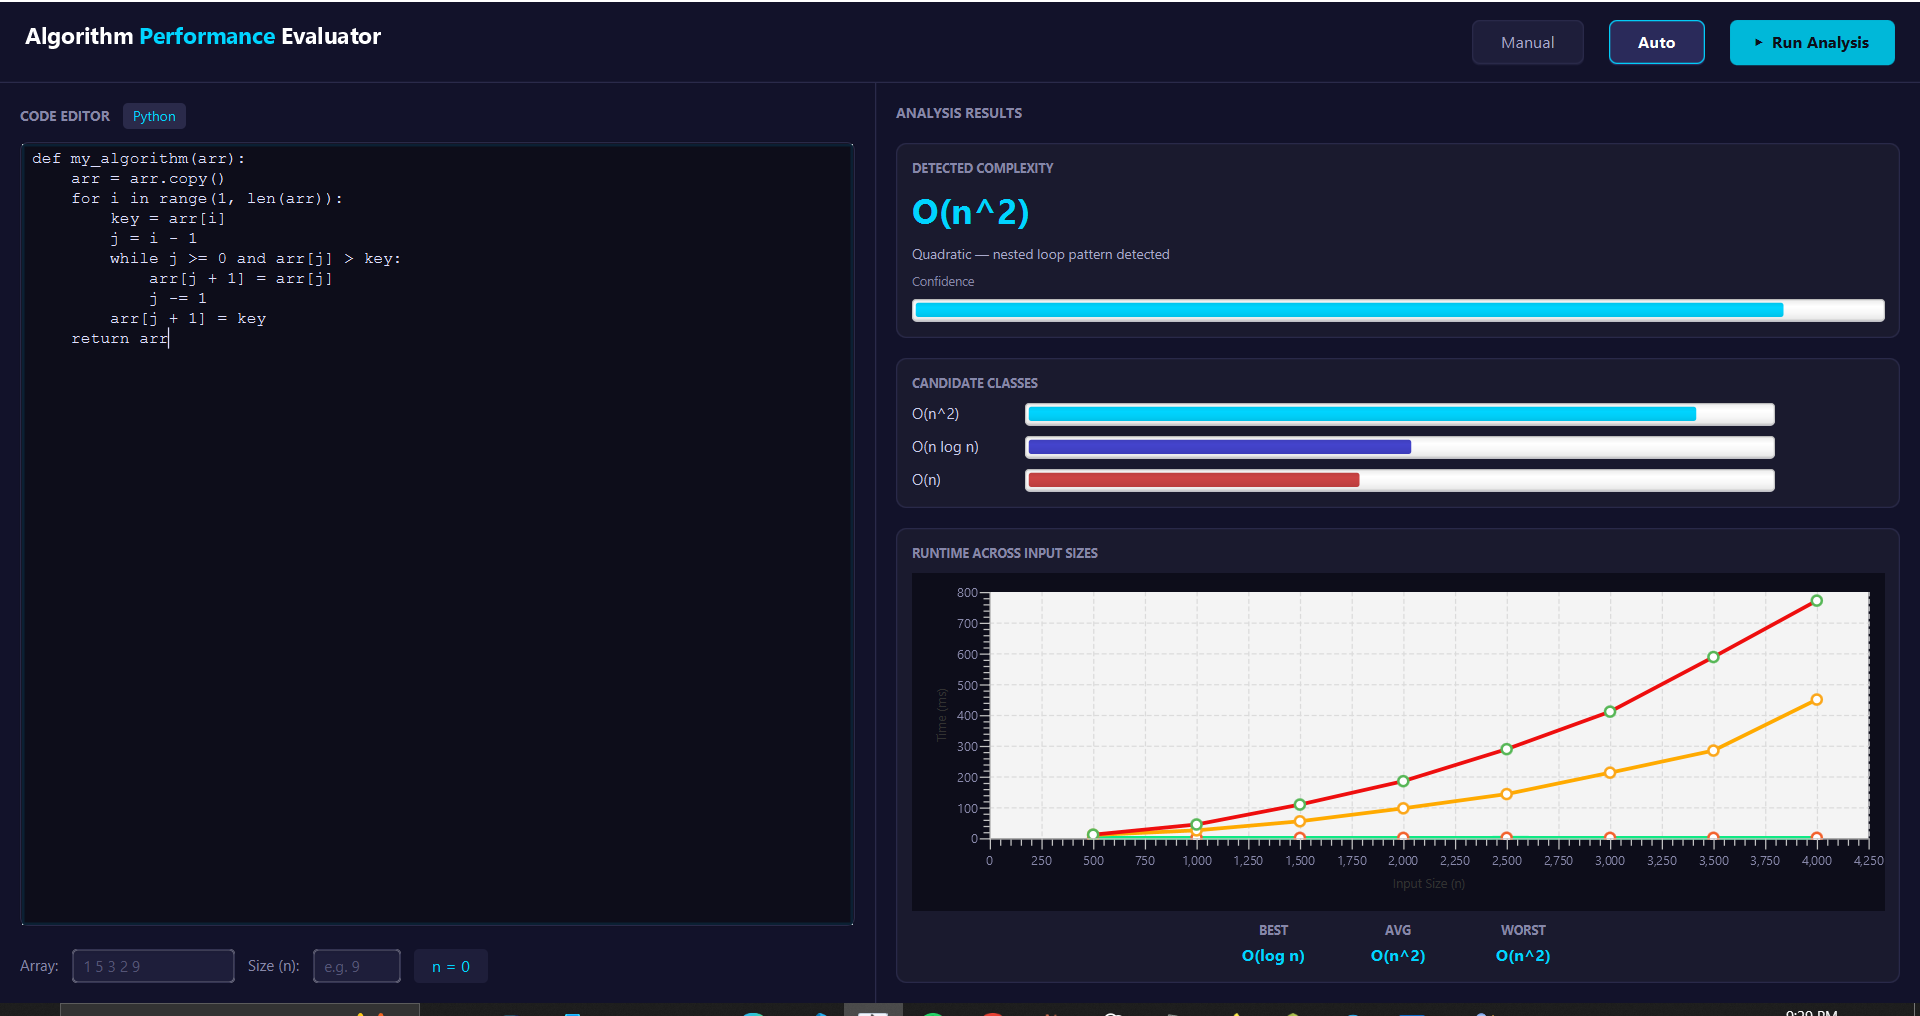
\includegraphics[width=0.9\textwidth]{../Assets/Insertion_Sort.png}
    \caption{Insertion Sort}
\end{figure}

\newpage
\subsection{Selection Sort}

\textbf{Code}
\begin{lstlisting}
    def my_algorithm(arr):
    arr = arr.copy()
    n = len(arr)
    for i in range(n):
        min_idx = i
        for j in range(i + 1, n):
            if arr[j] < arr[min_idx]:
                min_idx = j
        arr[i], arr[min_idx] = arr[min_idx], arr[i]
    return arr
\end{lstlisting}

\vspace{0.5cm}
\textbf{Result}
\begin{figure}[h]
    \centering
    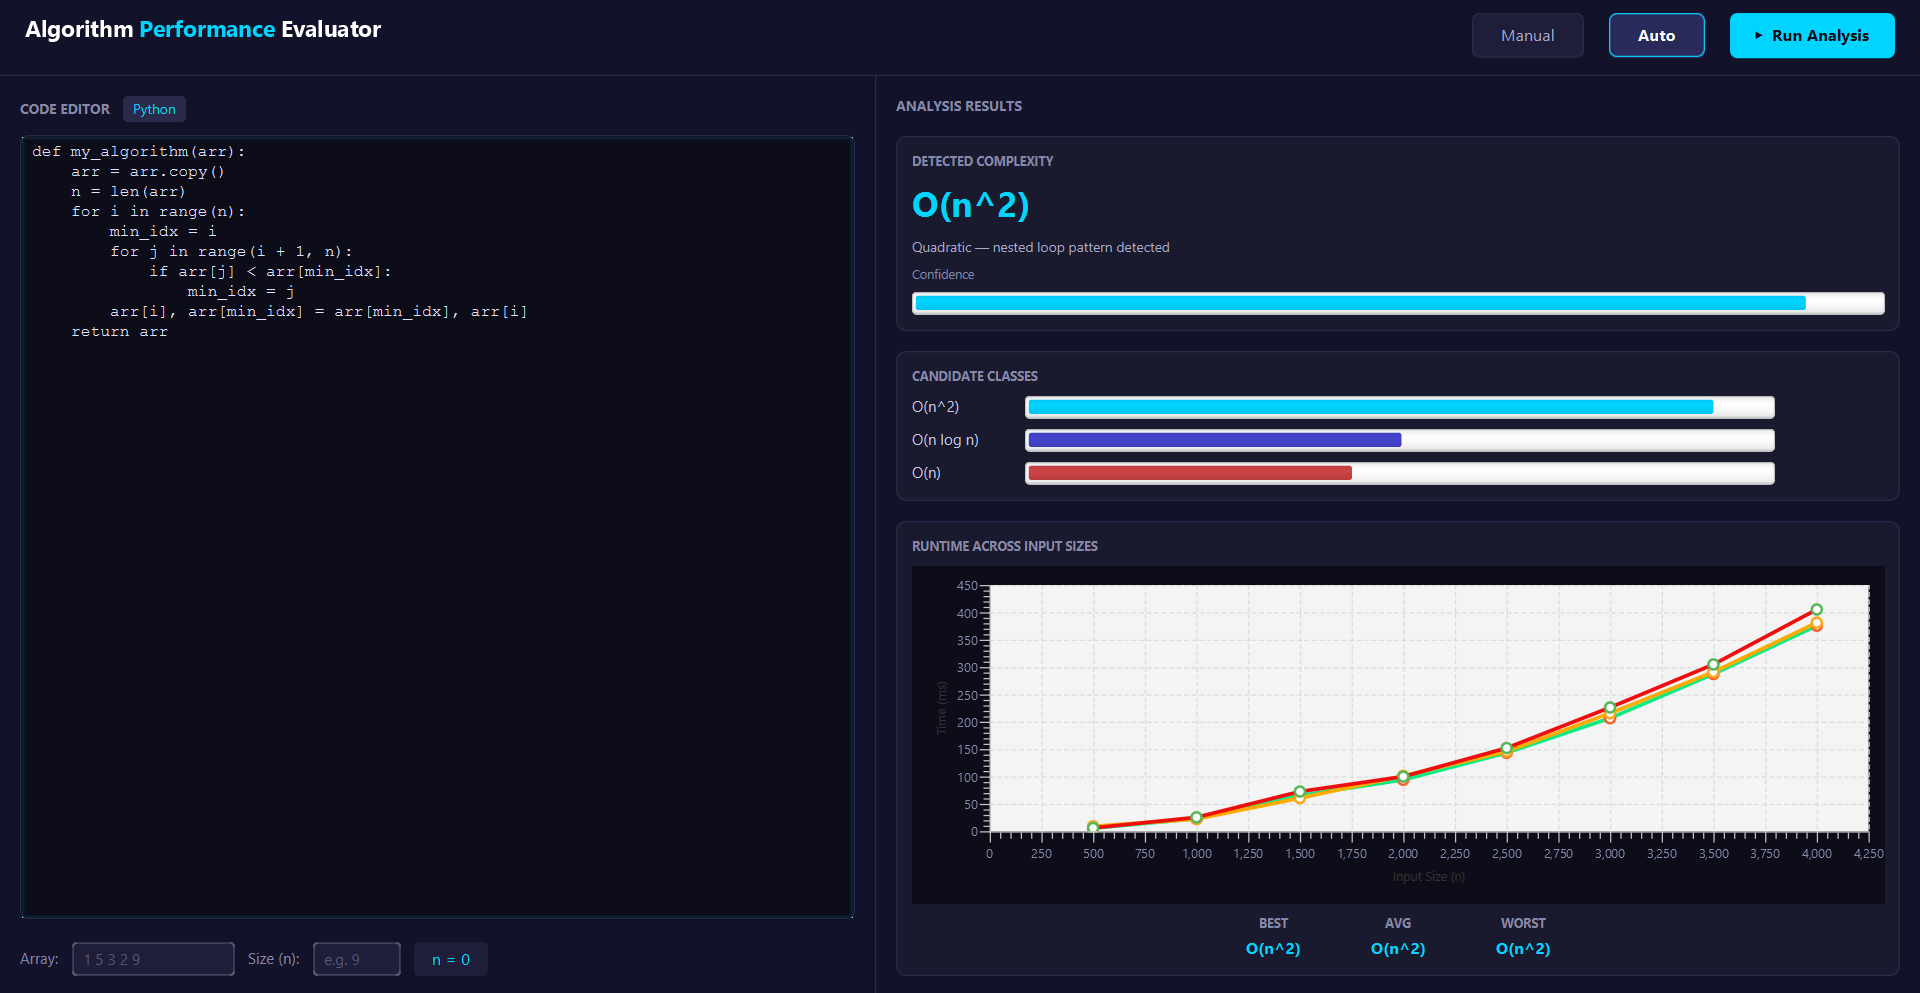
\includegraphics[width=0.9\textwidth]{../Assets/Selection_Sort.png}
    \caption{Selection Sort}
\end{figure}

\newpage
\subsection{Merge Sort}

\textbf{Code}
\begin{lstlisting}
    def my_algorithm(arr):
    arr = arr.copy()

    def merge_sort(a):
        if len(a) <= 1:
            return a
        mid = len(a) // 2
        left = merge_sort(a[:mid])
        right = merge_sort(a[mid:])
        return merge(left, right)

    def merge(left, right):
        result = []
        i = j = 0
        while i < len(left) and j < len(right):
            if left[i] <= right[j]:
                result.append(left[i])
                i += 1
            else:
                result.append(right[j])
                j += 1
        result.extend(left[i:])
        result.extend(right[j:])
        return result

    return merge_sort(arr)
\end{lstlisting}

\vspace{0.5cm}
\textbf{Result}
\begin{figure}[h]
    \centering
    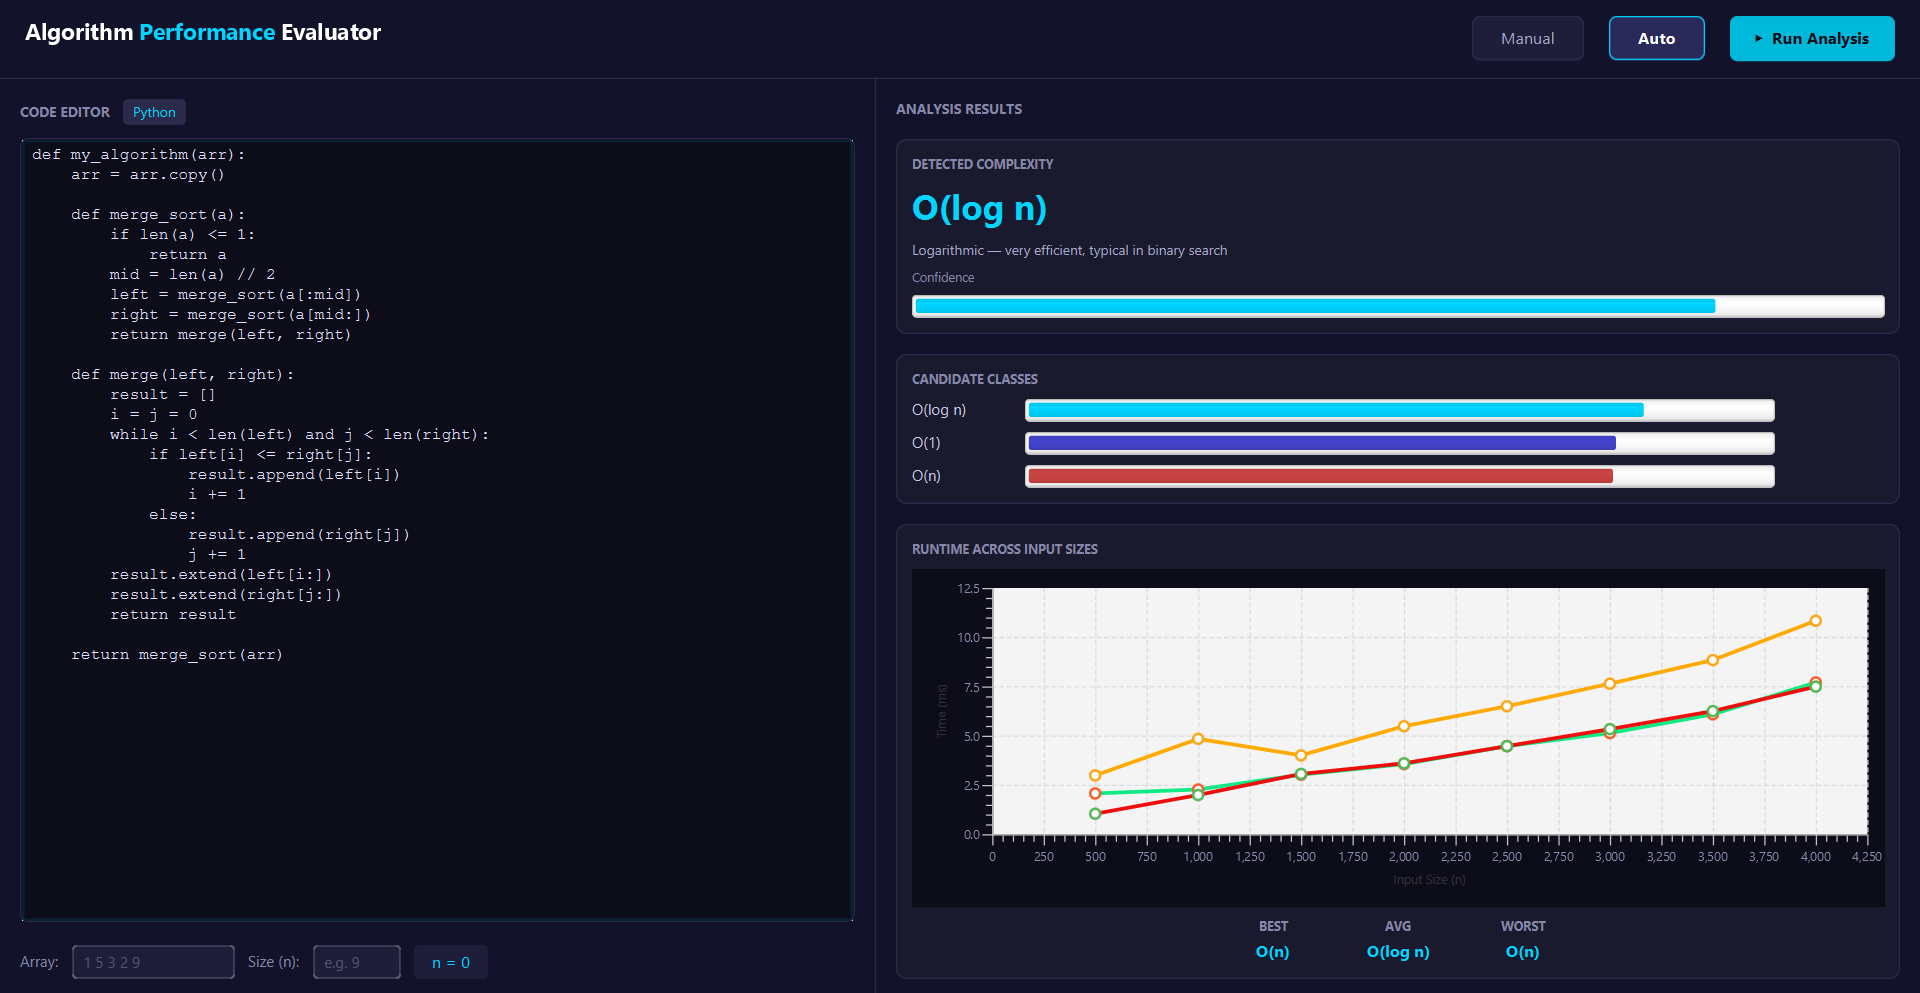
\includegraphics[width=0.9\textwidth]{../Assets/Merge_Sort.png}
    \caption{Merge Sort}
\end{figure}

\newpage
\subsection{Quick Sort}

\textbf{Code}
\begin{lstlisting}
    def my_algorithm(arr):
    arr = arr.copy()

    def quick_sort(a):
        if len(a) <= 1:
            return a
        pivot = a[len(a) // 2]

        left = [x for x in a if x < pivot]
        middle = [x for x in a if x == pivot]
        right = [x for x in a if x > pivot]
        return quick_sort(left) + middle + quick_sort(right)

    return quick_sort(arr)
\end{lstlisting}

\vspace{0.5cm}
\textbf{Result}
\begin{figure}[h]
    \centering
    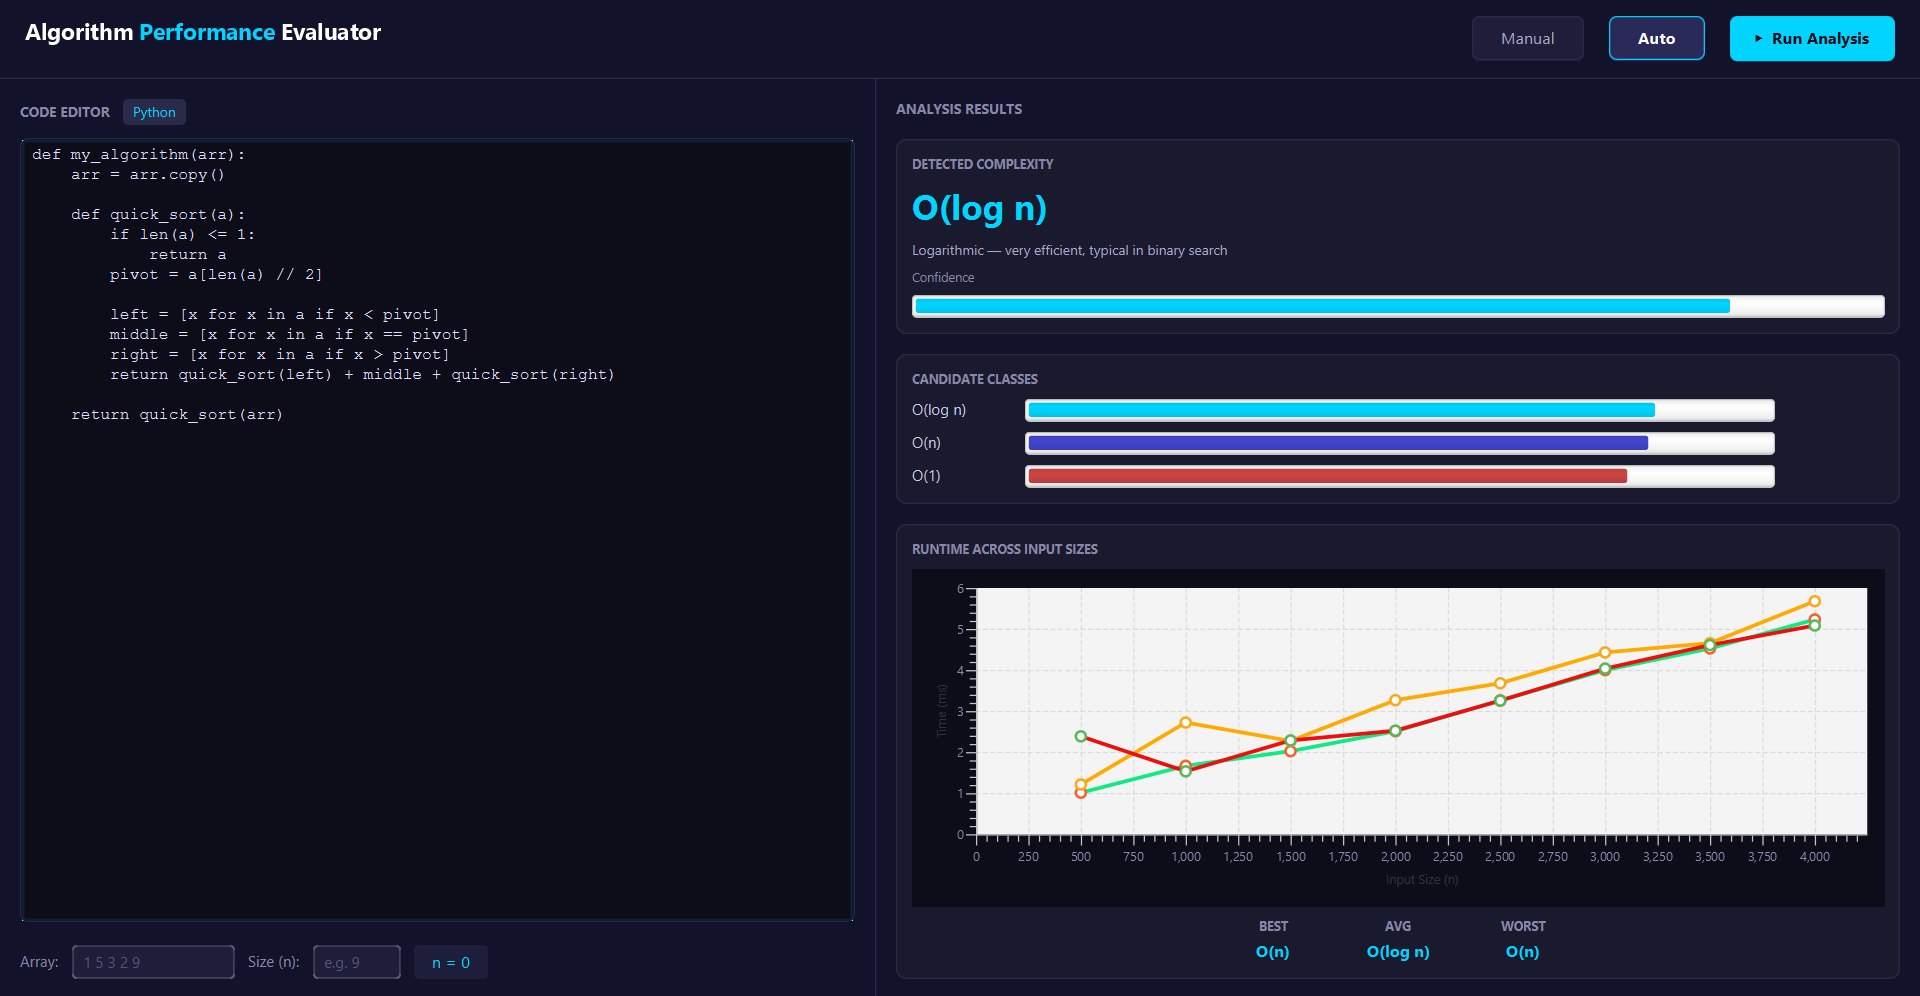
\includegraphics[width=0.9\textwidth]{../Assets/Qiuck_Sort.png}
    \caption{Quick Sort}
\end{figure}

\newpage
\section{References}

\begin{itemize}
\item Python Documentation: \url{https://docs.python.org/3/}
\item FastAPI Documentation: \url{https://fastapi.tiangolo.com/}
\item Java Documentation: \url{https://docs.oracle.com/en/java/}
\item JavaFX Documentation: \url{https://openjfx.io/}
\item Gson Library: \url{https://github.com/google/gson}
\item Big-O Complexity Overview: \url{https://www.geeksforgeeks.org/analysis-of-algorithms-set-1-asymptotic-analysis/}
\item Sorting Algorithms Reference: \url{https://www.geeksforgeeks.org/sorting-algorithms/}
\end{itemize}

\vspace{4cm}
\begin{center}
\textit{\Large Best Wishes}
\end{center}

\end{document}